\documentclass{article}

\usepackage{graphicx}
\usepackage{tikz}
\usepackage{tikzsymbols}
\usetikzlibrary{calc,patterns,shapes.geometric}
\pagestyle{empty}

\def\centerarc[#1](#2)(#3:#4:#5){\draw[#1] ($(#2)+({#5*cos(#3)},{#5*sin(#3)})$) arc (#3:#4:#5);}

\begin{document}
	\centering
	\begin{figure}
			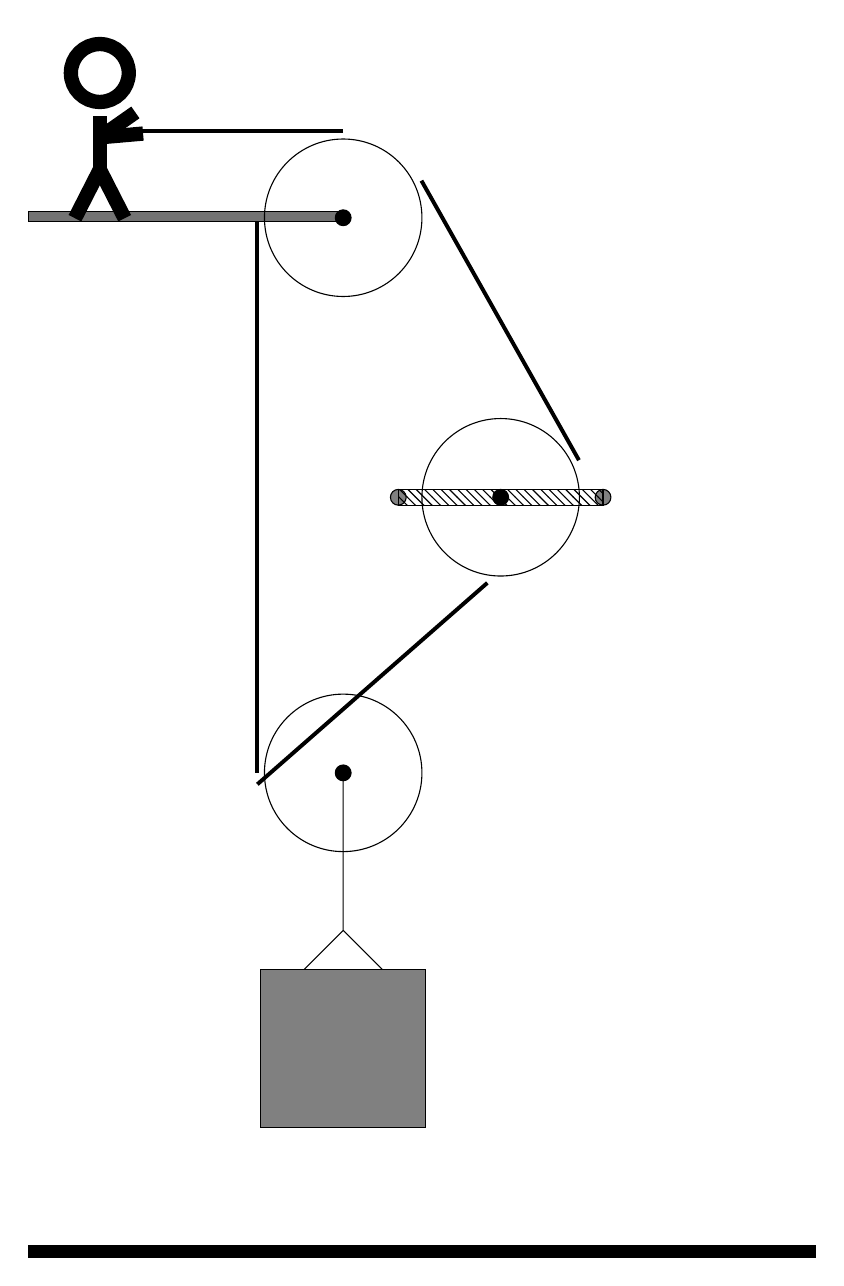
\begin{tikzpicture}
				%%%%% START %%%%%
								\draw[fill=black!55] (-2, 10) rectangle (2, 10.125);
				
				\draw (2, 3.0) circle (1);
				\draw[fill=black] (2, 3.0) circle (0.1);
				
				\draw (2, 10.05) circle (1);
				\draw[fill=black] (2, 10.05) circle (0.1);
				
				\draw[fill=white](4, 6.5) circle (1);
				\draw[fill=black] (4, 6.5) circle (0.1);
				\draw[fill=black!50] (2.7, 6.5) circle (0.1);
				\draw[fill=black!50] (5.3, 6.5) circle (0.1);
				\draw[pattern=north west lines, pattern color=black] (2.7, 6.6) rectangle (5.3, 6.4);
				
				\draw (2, 3.0) -- (2, 1.0) -- (1.5, 0.5) -- (2.5, 0.5) -- (2, 1.0);
				\draw[fill=black!50] (0.95, 0.5) rectangle (3.05, -1.5);
				
				\draw[line width=0.5mm] (0.9, 10) -- (0.9, 3.0);
				\centerarc[line width=0.5mm](2, 3.0)(180:330:1.1);
				\draw[line width=0.5mm](0.91, 2.855) -- (3.831, 5.413);
				\centerarc[line width=0.5mm](4, 6.5)(390:325:1.1);
				\draw[line width=0.5mm](4.994, 6.971) -- (2.994, 10.521);
				\centerarc[line width=0.5mm](2, 10.05)(30:90:1.1);
				\draw[line width=0.5mm](2, 11.15) -- (-1, 11.15);
				
				\node at (-1, 11.15) {\Strichmaxerl[10][-175][35]};
				
				\draw[fill=black] (-2, -3) rectangle (8, -3.15);
				%%%%% END %%%%%
			\end{tikzpicture}
	\end{figure}	
\end{document}